The upfront steps that were taken to create a shared understanding and to
examine possible solutions in building the application are shortly presented in
the current section.

\subsection{Determination of the Use Cases}
SmartCart in its final scope addresses two main use cases: the use case of
creating a shopping list and adding items to it as well as the process of going
shopping itself. The use case ``Go shopping�� implements the main user
interaction that consists of switching to the previous / next item and of
marking an item of the shopping list as �added to cart�. This interaction takes
place via gestures made by the user with its smartphone and detected by the
SmartCart application.

\begin{figure}
\centering
\captionsetup{justification=centering}
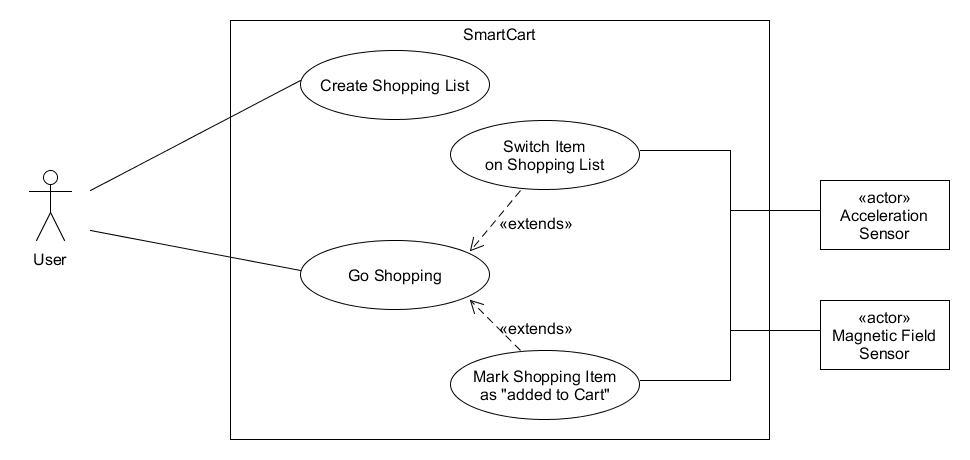
\includegraphics[width=\textwidth]{res/sa/useCaseDiagram.png}
\caption{Overview of the System's Use Cases}
\label{fig:UseCases}
\end{figure}

\subsection{Relations between the captured Gestures
and the used Sensors}

\begin{figure}
\centering
\captionsetup{justification=centering}
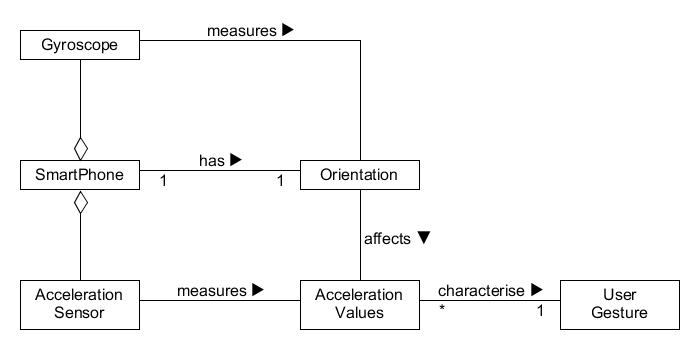
\includegraphics[width=\textwidth]{res/sa/UserGestureDataModel.png}
\caption{Data Model of the User Gestures to recognize}
\label{fig:UseCases}
\end{figure}